\chapter{Requirements}
\section{Allgemeine Beschreibung}
\subsection{Produktperspektive}
Mit Internet of Things sind eine Vielzahl neuartige Devices entstanden. Während in herkömmlichen Netzwerken hauptsächlich Personal Computer, Notebooks, Server usw. verwaltet werden mussten, so bringen IoT Devices den IT-Abteilungen neue Herausforderungen. Zum einen dürfte die Anzahl Geräte gegenüber herkömmlichen Computer deutlich ansteigen, zum anderen sind IoT Devices in Sachen Funktionalität und Rechenleistung, sowie auch der Netzwerkbandbreite deutlich beschränkt. 

Mit dieser Arbeit soll eine Management Applikation bereitgestellt werden, um eine Vielzahl unterschiedlicher IoT Devices administrieren zu können. 
\subsection{Produktfunktionen}
Die Applikation soll den Benutzern erlauben, IoT Geräte zu verwalten. Die Aufgaben reichen vom Erfassen und Discovery von Devices über die Konfigurationsverwaltung und Softwareverteilung bis zu Backup und Restore. Ausserdem sollen Management-relevante Kommandos auf Devices ausgeführt- und Security Aspekte beachtet werden. Die Details zu den Produktfunktionen sind den Use Cases zu entnehmen.

\subsection{Benutzer Charakteristik}
Zielpersonen der Applikation sind Betreiber von IoT Devices. Dies können im Enterprise Umfeld IT-Mitarbeiter in operationeller Funktion-, oder auch Softwareentwickler für IoT Applikationen sein. Heimanwender können bei entsprechenden Kenntnissen ebenfalls zur Zielgruppe gehören. Es werden solide Grundkenntnisse in TCP/IP Netzwerken sowie Verständnis der verwendeten IoT Architekturen und Devices vorausgesetzt. 
\section{Use Cases}
\subsection{Use Cases Diagramm}
\begin{figure}[H]
\centering
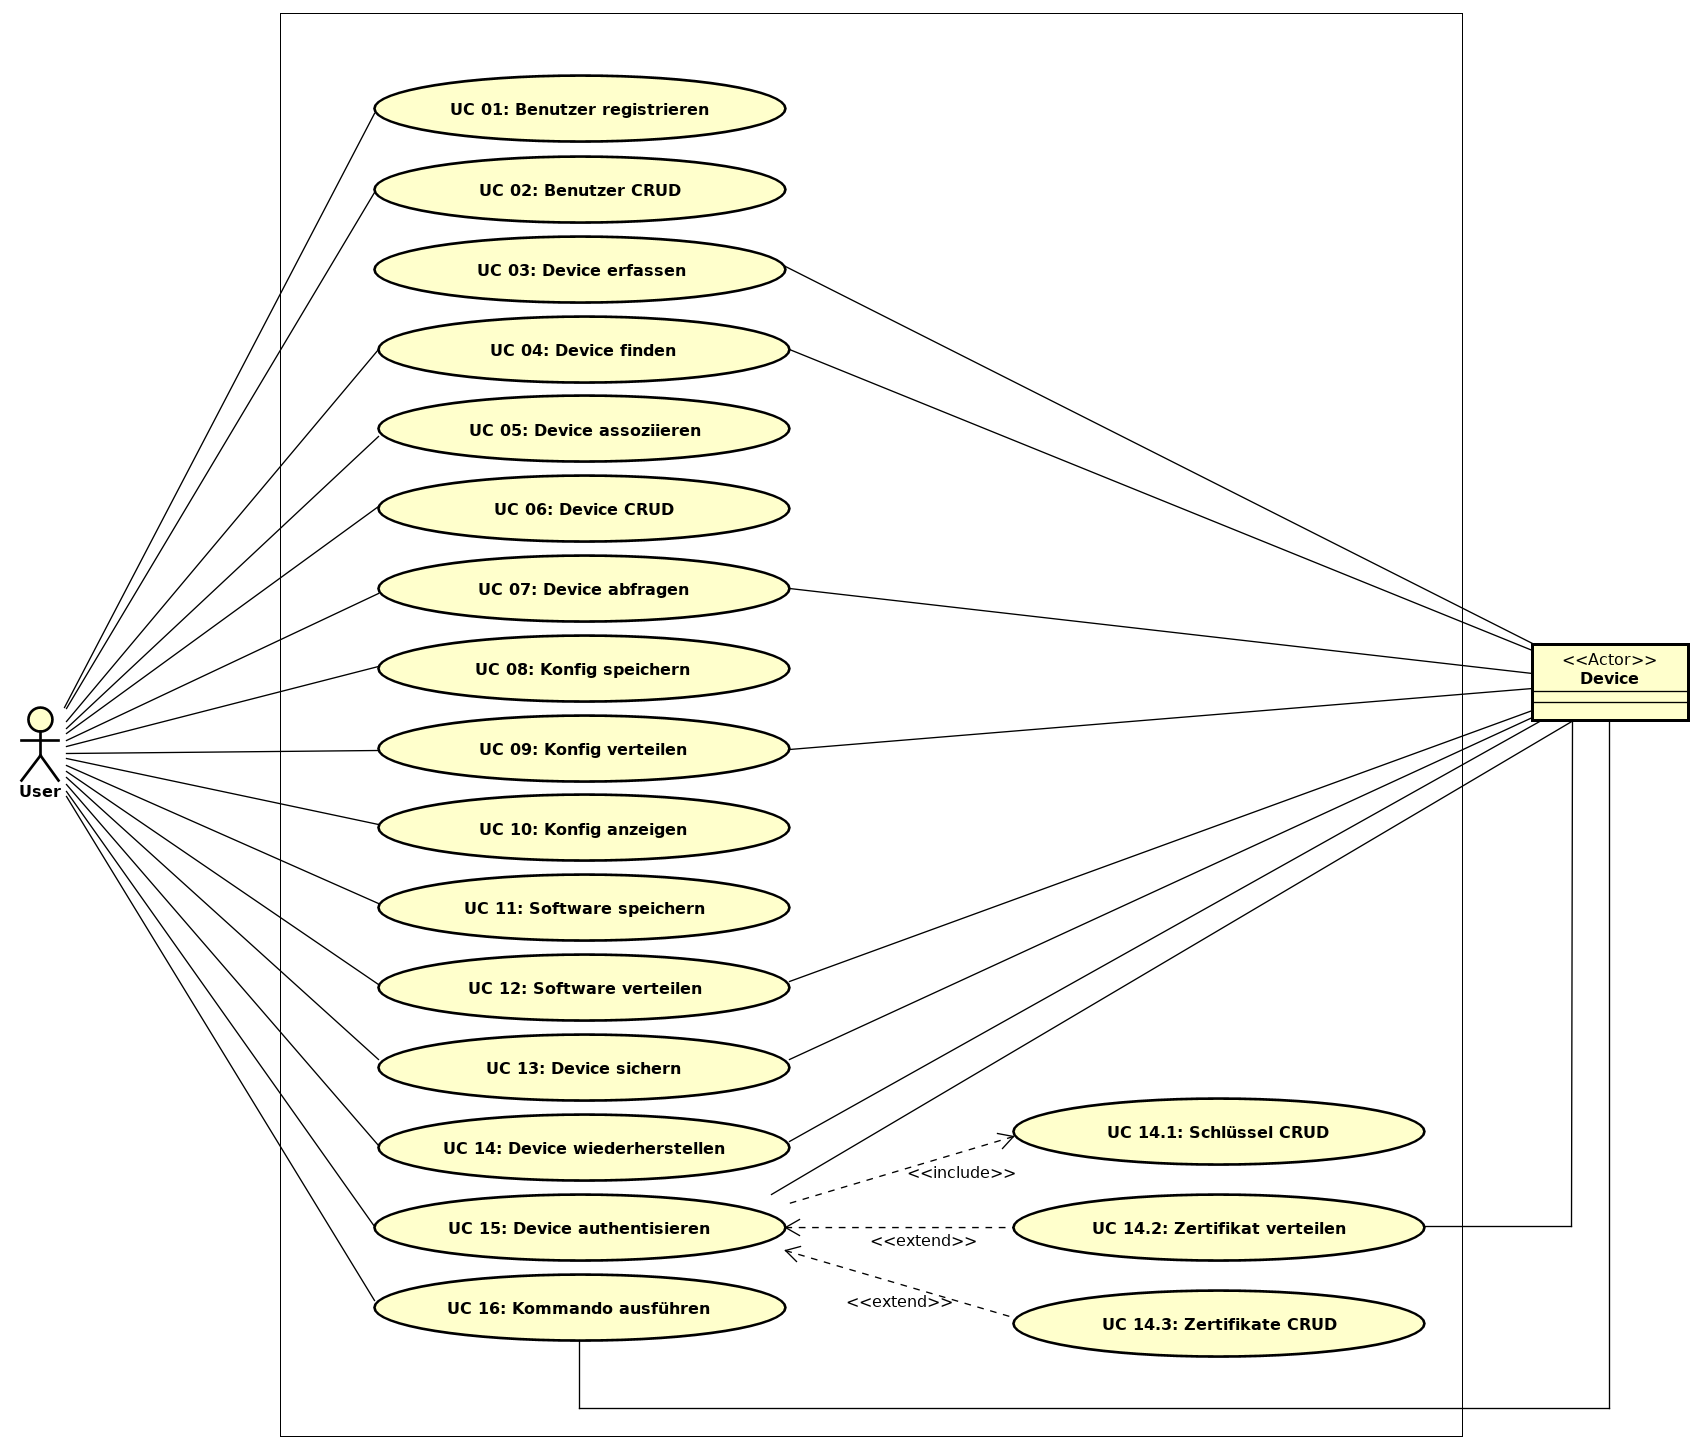
\includegraphics[scale=0.39]{images/use_case_diagram.png}\caption{Use Case Diagramm}
\end{figure}
\newpage
\subsection{Priorisierung}
Da die Umsetzung aller Use Cases den Rahmen einer Bachelorarbeit sprengen würde, wurden die diese wie folgt priorisiert:
\begin{center}
\begin{longtable}{| p{5.5cm} | p{3cm} |}
\hline
\textbf{Use Case} & \textbf{Priorität}\\ \hline
UC 01: Benutzer registrieren     & Optional \\ \hline
UC 02: Benutzer login			 & Optional \\ \hline
UC 03: Benutzer CRUD	         & Optional \\ \hline 
UC 04: Device CRUD               & Pflicht \\ \hline 
UC 05: Device finden			 & Pflicht \\ \hline 
UC 06: Device authentisieren     & Pflicht \\ \hline
UC 07: Device verbinden			 & Pflicht \\ \hline
UC 08: File CRUD				 & Pflicht \\ \hline
UC 09: Device sichern			 & Pflicht \\ \hline
UC 10: Device wiederherstellen	 & Optional \\ \hline
UC 11: Kommando ausführen		 & Pflicht \\ \hline  
\end{longtable}
\end{center}
\subsection{Aktoren}
Der Benutzer der Applikation ist in diesem System der einzige primäre Aktor. Dieser bewirtschaftet die Applikation und verwaltet alle Devices und Benutzer. Als Sekundärer Aktor werden die einzelnen Devices gezählt.
\newpage
\subsection{Beschreibungen (Casual)}
\subsubsection{Benutzer registrieren}
\mbox{}
\begin{longtable}{| p{4cm} | p{11.7cm} |}
 \hline
 \textbf{ID} & 01\\ \hline 
 \textbf{Name} & Benutzer registrieren\\ \hline 
 \textbf{Beschreibung} & Der Benutzer legt sich einen neuen Account für die Management Software an.\\ \hline 
 \textbf{Preconditions} & 
   \tabitem Applikation gestartet
  \\ \hline 
 \textbf{Postconditions} & 
  \tabitem Neuer Benutzer ist gespeichert
 \\ \hline
 \textbf{Main Success Scenario} &
 1. Benutzer wählt ''Benutzer registrieren'' \newline
 2. Benutzer gibt Loginangaben ein \newline
 3. Benutzer speichert die Eingaben
\\  \hline 
 \textbf{Extensions} & -\\ \hline 
 \end{longtable}
 
\subsubsection{Benutzer login}
\mbox{}
\begin{longtable}{| p{4cm} | p{11.7cm} |}
 \hline
 \textbf{ID} & 02\\ \hline 
 \textbf{Name} & Benutzer login\\ \hline 
 \textbf{Beschreibung} & Der Benutzer loggt sich in der Applikation ein.\\ \hline 
 \textbf{Preconditions} & 
   \tabitem Applikation gestartet
   \tabitem Benutzer im System angelegt
  \\ \hline 
 \textbf{Postconditions} & 
  \tabitem Benutzer kann auf dem Management Startseite interagieren.
 \\ \hline
 \textbf{Main Success Scenario} &
 1. Loginseite erscheint beim Start der Applikation \newline
 2. Benutzer gibt Benutzername und Passwort ein \newline
 3. Benutzer wählt \glqq Login\grqq . \newline
 4. Benutzer ist eingeloggt.
\\  \hline 
 \textbf{Extensions} & 
 4.a Fehlermeldung bei falschem Login erscheint.   
 \\ \hline 
 \end{longtable}



\subsubsection{Benutzer CRUD}
\mbox{}
\begin{longtable}{| p{4cm} | p{11.7cm} |}
 \hline
 \textbf{ID} & 03\\ \hline 
 \textbf{Name} & Benutzer CRUD\\ \hline 
 \textbf{Beschreibung} & Benutzerverwaltung der Applikation\\ \hline 
 \textbf{Preconditions} & 
   \tabitem Applikation gestartet \newline
   \tabitem Benutzer ist registriert \newline
   \tabitem Benutzer ist eingeloggt 
  \\ \hline 
 \textbf{Postconditions} & 
  \tabitem Änderungen gespeichert
 \\ \hline
 \textbf{Main Success Scenario} &
 \textbf{Create:}\newline
  1. UC 01: Benutzer registrieren \newline
 \textbf{Read:}\newline
  1. Benutzer lässt Userdaten anzeigen \newline
 \textbf{Update:}\newline
  1. Benutzer lässt Userdaten anzeigen \newline
  2. Benutzer verändert Attribute\newline
  3. Benutzer speichert Änderungen\newline
 \textbf{Delete:}\newline
  1. Benutzer wird gelöscht \\ 
 \hline 
 \textbf{Extensions} & -\\ \hline 
 \end{longtable}
\newpage

\subsubsection{Device CRUD}
\mbox{}
\begin{longtable}{| p{4cm} | p{11.7cm} |}
 \hline
 \textbf{ID} & 04\\ \hline 
 \textbf{Name} & Device erfassen \\ \hline 
 \textbf{Beschreibung} & Der Benutzer möchte ein Device manuell hinzufügen. Der Endpunkt ist dem Benutzer bekannt. 
 \\ \hline 
 \textbf{Preconditions} & 
   \tabitem Applikation gestartet \newline
   \tabitem Benutzer eingeloggt \newline
   \tabitem Device Endpunkt ist dem Benutzer bekannt
  \\ \hline 
 \textbf{Postconditions} & 
  \tabitem Falls ein Gerät gefunden wird, wird es angezeigt 
  \\ \hline 
 \textbf{Main Success Scenario} & 
  \textbf{Create:}\newline
  1. Benutzer wählt \glqq Device erfassen\grqq . \newline
  2. Benutzer erfasst Daten im Formular. \newline
  3. Benutzer wählt \glqq erfassen\grqq . \newline
 \textbf{Read:}\newline
  1. Benutzer navigiert zur Geräteübersicht \newline
  2. Device details werden angezeigt \newline
 \textbf{Update:}\newline
  1. Benutzer navigiert zur Geräteübersicht \newline
  2. Benutzer passt Geräteinformationen an. \newline
  3. Benutzer wählt \glqq erfassen\grqq . \newline
 \textbf{Delete:}\newline
  1. Benutzer navigiert zur Geräteübersicht \newline
  2. Benutzer wählt \glqq delete\grqq . \newline
  3. Gerät wird vom System gelöscht.
  \\ \hline 
 \textbf{Extensions} & 
  \textbf{Read:}\newline
  3. Benutzer wählt \glqq Read\grqq . \newline
  4. Aktualisierte Device Informationen werden angezeigt.
  \\ \hline 
\end{longtable}
\subsubsection{Device finden}
\mbox{}
\begin{longtable}{| p{4cm} | p{11.7cm} |}
 \hline
 \textbf{ID} & 05\\ \hline 
 \textbf{Name} & Device finden\\ \hline 
 \textbf{Beschreibung} & Der Benutzer möchte ein- oder meherere Devices finden. Endpunkt des Devices ist dem Benutzer unbekannt. Gefundene Devices sollen dem Benutzer aufgelistet werden. \\ \hline 
 \textbf{Preconditions} &  
  \tabitem Applikation gestartet \newline
  \tabitem Benutzer eingeloggt
 \\ \hline 
 \textbf{Postconditions} & 
  \tabitem Gefundene Devices werden dem Benutzer angezeigt 
 \\ \hline 
 \textbf{Main Success Scenario} & 
  1. Benutzer öffnet Device Discovery \newline
  2. System listet eingegangene Anfragen von Devices auf \newline
 \\ \hline 
 \textbf{Extensions} &  
  2.a System zeigt Fehlermeldung an
 \\ \hline 
 \end{longtable}

\newpage
\subsubsection{Device authentisieren}
\mbox{}
\begin{longtable}{| p{4cm} | p{11.7cm} |}
 \hline
 \textbf{ID} & 06\\ \hline 
 \textbf{Name} & Device authentisieren\\ \hline 
 \textbf{Beschreibung} & Anmeldung am Device\\ \hline 
 \textbf{Preconditions} &  
  \tabitem Applikation gestartet \newline
  \tabitem Benutzer eingeloggt \newline
  \tabitem Device im System erfasst \newline
  \tabitem Authentisierungsdaten im Device erfasst \newline
  \tabitem Verbindung zum Device möglich
 \\ \hline 
 \textbf{Postconditions} & - 
 \\ \hline 
 \textbf{Main Success Scenario} & 
  1. Benutzer wählt Aktion (Read, etc.) auf Device \newline
  2. System baut Verbindung zu Device auf \newline
  3. System authentifiziert sich am Device \newline
  4. Benutzer erhält Feedback über Authentisierung
 \\ \hline 
 \textbf{Extensions} & 
  2.a Verbindungsfehler
  3.a Authentifizierungsfehler
 \\ \hline 
 \end{longtable}

\subsubsection{Device verbinden}
\mbox{}
\begin{longtable}{| p{4cm} | p{11.7cm} |}
 \hline
 \textbf{ID} & 07\\ \hline 
 \textbf{Name} & Device verbinden\\ \hline 
 \textbf{Beschreibung} & Kommunikation mit Device erstellen\\ \hline 
 \textbf{Preconditions} &  
  \tabitem Applikation gestartet \newline
  \tabitem Benutzer eingeloggt \newline
  \tabitem Device im System erfasst \newline
 \\ \hline 
 \textbf{Postconditions} & - 
 \\ \hline 
 \textbf{Main Success Scenario} & 
  1. Benutzer wählt Aktion (Read, etc.) auf Device \newline
  2. System baut Verbindung zu Device auf \newline
  3. Benutzer erhält Feedback über Verbindungsaufbau
 \\ \hline 
 \textbf{Extensions} & 
  2.a Verbindungsfehler
  \\ \hline 
 \end{longtable}

\newpage
\subsubsection{File CRUD}
\mbox{}
\begin{longtable}{| p{4cm} | p{11.7cm} |}
 \hline
 \textbf{ID} & 08\\ \hline 
 \textbf{Name} & File CRUD\\ \hline 
 \textbf{Beschreibung} &  Files für Devices können im System verwaltet werden\\ \hline 
 \textbf{Preconditions} &
  \tabitem Applikation gestartet \newline
  \tabitem Benutzer eingeloggt \newline
 \\ \hline 
 \textbf{Postconditions} & -
 \\ \hline 
 \textbf{Main Success Scenario} &
 \textbf{Create:} \newline
 \tabitem Benutzer wählt \glqq File upload\grqq . \newline
 \tabitem Benutzer selektiert File aus lokalem Dateisystem. \newline
 \tabitem File wird im System abgelegt. \newline
 \tabitem Benutzer erhält Feedback über Erfolg. \newline
 \textbf{Read:} \newline
 \tabitem Benutzer wählt File auf System. \newline
 \tabitem Benutzer wählt \glqq show file\grqq . \newline
 \textbf{Update:} \newline
 \tabitem Benutzer wählt File auf System. \newline
 \tabitem Benutzer wählt \glqq edit file\grqq .\newline
 \tabitem Benutzer passt Dateiinhalt an. \newline
 \tabitem Benutzer speichert Änderungen.
 \textbf{Delete:} \newline 
 \tabitem Benutzer wählt File auf System. \newline
 \tabitem Benutzer wählt \glqq delete\grqq . \newline
 \tabitem File wird von System gelöscht. \newline
 \\ \hline 
 \textbf{Extensions} &
  
 \\ \hline 
 \end{longtable}

\newpage
\subsubsection{Device sichern}
\mbox{}
\begin{longtable}{| p{4cm} | p{11.7cm} |}
 \hline
 \textbf{ID} & 09\\ \hline 
 \textbf{Name} & Device sichern\\ \hline 
 \textbf{Beschreibung} & Von den Devices können Sicherungen gemacht werden, welche den Software- sowie den Konfigurationsstand beinhalten. Diese Sicherungen werden gespeichert. \\ \hline 
 \textbf{Preconditions} & 
  \tabitem Applikation gestartet\newline
  \tabitem Benutzer ist eingeloggt \newline
  \tabitem Devices assoziiert (UC 5) \\ \hline
 \textbf{Postconditions} & 
  \tabitem Sicherung des Gerätes sind gespeichert
 \\ \hline 
 \textbf{Main Success Scenario} &
  1. Benutzer selektiert das betreffende Device aus. \newline
  2. ''Device sichern'' wird ausgewählt\newline
  3. Die Sicherung wird benannt und ein Datum wird vergeben \newline
  4. ''Sind Sie sich sicher?''-Abfrage wird angezeigt\newline
  5. Sicherungsvorgang wird gestartet\newline
  6. Sicherung wird heruntergeladen\newline
  7. Device Feedback anzeigen\newline
  8. Sicherung wird gespeichert
 \\ \hline 
 \textbf{Extensions} &
  1.a Benutzer selektiert mehrere Geräte. \newline
  3.a Fehlermeldung wird angezeigt, da der gleiche Name schon vorhanden ist\newline
  4.a Abfrage wird verneint -> Vorgang wird abgebrochen\newline
  6.a I/O Fehlermeldung \newline
  7.a Timeout wird erreicht.\newline
  7.b Fehlermeldungen zu der Wiederherstellung wird angezeigt. \newline
  8.a I/O Fehlermeldung
 \\ \hline 
 \end{longtable}
\newpage
\subsubsection{Device wiederherstellen}
\mbox{}
\begin{longtable}{| p{4cm} | p{11.7cm} |}
 \hline
 \textbf{ID} & 10\\ \hline 
 \textbf{Name} & Device wiederherstellen\\ \hline 
 \textbf{Beschreibung} & Das Device muss wiederhergestellt werden. Dadurch wird ein Software- sowie Konfigurationsstand auf das Device geschrieben. \\ \hline 
 \textbf{Preconditions} & 
  \tabitem Applikation gestartet\newline
  \tabitem Benutzer ist eingeloggt \\ \hline
 \textbf{Postconditions} & - \newline
  \tabitem Das Gerät funktioniert korrekt\newline
  \tabitem Das Gerät hat den richtigen Softwarestand\newline
  \tabitem Das Gerät hat die richtige Konfiguration
  \\ \hline 
 \textbf{Main Success Scenario} & 
  1. Benutzer selektiert das betreffende Device aus. \newline
  2. ''Device wiederherstellen'' wird ausgewählt\newline
  3. Backups für das Device werden angezeigt\newline
  4. Backup wird selektiert\newline
  5. ''Sind Sie sich sicher?''-Abfrage wird angezeigt\newline
  6. Wiederherstellungsvorgang wird gestartet\newline
  7. Device Feedback anzeigen
 \\ \hline 
 \textbf{Extensions} &
  1.a Benutzer selektiert mehrere Geräte. \newline
  3.a Fehlermeldung, da keine Backups vorhanden sind\newline
  5.a Abfrage wird verneint -> Vorgang wird abgebrochen\newline
  7.a Timeout wird erreicht.\newline
  7.b Fehlermeldungen zu der Wiederherstellung wird angezeigt. 
 \\ \hline 
 \end{longtable}

\subsubsection{Kommandos ausführen}
\mbox{}
\begin{longtable}{| p{4cm} | p{11.7cm} |}
 \hline
  \textbf{ID} & 11\\ \hline 
 \textbf{Name} & Kommandos ausführen\\ \hline 
 \textbf{Beschreibung} & Dem Gerät werden Kommandos, wie zum Beispiel ''Reboot'' oder ''Shutdown'', gesendet.\\ \hline 
 \textbf{Preconditions} & 
  \tabitem Applikation gestartet\newline
  \tabitem Benutzer ist eingeloggt \\ \hline
 \textbf{Postconditions} & \newline
 \tabitem Kommandos sind ausgeführt \newline
 \tabitem Device Feedback
 \\ \hline
 \textbf{Main Success Scenario} &
  1. Benutzer selektiert das betreffende Device aus. \newline
  2. Das auszuführende Kommando wird gewählt/eingegeben \newline
  3. Das Kommando wird an alle ausgewählten Devices gesendet \newline
  4. Devicefeedback wird angezeigt. \\ \hline 
 \textbf{Extensions} &
 1.a Benutzer selektiert mehrere Geräte. \newline
 4.a Fehlermeldungen zu dem Kommando werden angezeigt. \newline
 4.b Timeout wird erreicht. \\ \hline 
\end{longtable}
\newpage
\section{Nichtfunktionale Anforderungen}
In diesem Kapitel werden die nicht funktionalen Anforderungen des Projekt aufgezeigt. Wir behandeln Aspekte und Anforderungen aus den Bereichen Qualität, Schnittstellen und Randbedingungen.
\subsection{Qualität}
Bei der Softwarequalität stützen wir uns auf die ISO/IEC 9126 Norm. Es werden die Merkmale Funktionalität, Zuverlässigkeit, Benutzbarkeit, Effizienz, Wartbarkeit und Übertragbarkeit aufgeführt. 
\subsubsection{Funktionalität}
IoT Devices können von vielen unterschiedlichen Herstellern kommen. Devices können somit sehr unterschiedliche Attribute enthalten. Ebenfalls können sich die Art der Kommunikation und unterstützte Netzwerkprotokolle unterscheiden. Um die Funktionalität bestmöglich sicherzustellen, wird die Herstellerunterstützung vorerst stark eingeschränkt.
\subsubsection{Zuverlässigkeit}
Eine Managementplattform von IoT Devices ist nicht Realtime-kritisch. Bei einem Ausfall der Managementplattform, würde das nicht zu einem Schwerwiegenden Problem führen, da die Geräte trotzdem weiterarbeiten könnten. Für die Provisionierung, Fehlersuche oder Updateprozesse ist das Managementtool aber unerlässlich

Durch die vielseitigen Aufgaben muss auf die Parallelität geachtet werden. Es werden durchaus zeitintensive Tasks ausgeführt, welche potenziell die Applikation über längere Zeit blockieren könnten.
\subsubsection{Benutzbarkeit}
Um eine simple Bedienung zu gewährleisten soll eine einfache und zweckmässige Benutzeroberfläche zur Verfügung gestellt werden.
\subsubsection{Effizienz}
Die Effizienz hängt stark von den IoT Devices, deren Internetbandbreite und Rechenleistung ab.
\subsubsection{Wartbarkeit}
Sämtliche Teile der Software sollen möglichst modular und lose gekoppelt aufgebaut werden. Eine Management-Applikation für IoT könnte potenziell sehr umfangreich sein und eine Weiterentwicklung muss in Betracht gezogen werden. Auch muss der gesamte Codeumfang verständlich sein oder mit allfälligen Kommentaren/Dokumentationen beschrieben sein.
\subsubsection{Übertragbarkeit}
Die Applikation soll für Clients über gängige Webbrowser zugänglich sein. Deshalb sollte eine Übertragbarkeit auf verschiedene Clientsysteme keine Probleme darstellen.
\subsection{Schnittstellen}
\subsubsection{Benutzerschnittstellen}
Die Steuerung des Programms ist über eine grafische Weboberfläche vorgesehen. Tastatur und Maus sind notwendig.
\subsubsection{Netzwerkschnittstellen}
Um die Applikation zu bedienen benötigt der Client einen funktionierenden Internetanschluss. Die Applikation selbst muss ebenfalls über einen Internetzugang verfügen und die nötigen Kommunikationsports müssen geöffnet sein.
\subsection{Sicherheit}
Da die Applikation über das Internet erreichbar ist, muss die Applikationssicherheit gewährleistet sein. Eine Kompromittierung der Management Plattform könnte die gesamte IoT Landschaft eines Unternehmens beeinträchtigen. Man könnte beispielsweise Geräte herunterfahren oder mit bösartiger Malware ausstatten. Es gilt unbedingt die Grundregeln der Informationssicherheit einzuhalten. Sämtliche Zugriffe sollen autorisiert- und vertrauliche Informationen verschlüsselt übertragen werden.